

\documentclass[main.tex]{subfiles}

\begin{document}


\chapter{Introduction}

\section{What is this course about?}

\mnote{Composite} 
The aim of the course is to provide a unified view to the 
behavior of materials and structures made of composites that combine 
brittle matrix with tensile reinforcement.
The term "composite" denotes a material made up of constituent materials that play different roles in the material behavior.
In cementitious composites the constituents are specialized on compressive and tensile behavior.
The concrete matrix material with high compressive strength surrounds and supports the relative position of the reinforcement material (steel, carbon or glass) with high tensile strength.

The term "brittle" implies a 
\mnote{Brittle matrix}
sudden local failure that is observed as 
a distinguished fracture of material. In the usual sense, this property is associated 
with glass, ceramics and carbon. Such materials exhibit perfectly 
elastic deformation and sudden failure.

\mnote{Behavior of concrete} 
To large extent, concrete and cementitious matrices can also be regarded
as brittle. Upon tensile stresses, a macroscopically observable cracks develop 
that initiate a sudden failure. However, in comparison to the brittle materials
mentioned above, the material structure of concrete is consisting of coarse 
aggregates and cement paste, the process of cracking is more complex.
The evolution of a macroscopically observable crack involves a coalescence of  microcracks, a process that is not purely elastic-brittle. It is governed by local dissipative mechanisms of internal friction
and sliding between aggregates at the scale of the material structure.
Such kind of gradual material disintegration is specific to concrete.
The local failure is not a sudden event but gradual process 
involving the development of microcracks and their localization to a macrocrack.
Phenomenologically, this process leads to nonlinear stress-strain behavior. In fact, concrete is neither elastic, nor plastic and even not purely brittle.
It is something in-between so that its material behavior is  referred to as "quasi-brittle". 
The complexity of the crack localization process makes a
an objective general description of concrete material behavior a challenging task and remains a subject of an ongoing research.

\mnote{Behavior of reinforced concrete}
Simply speaking, one could say, that the only reason for putting steel into concrete
is to prevent the failure upon the appearance of a crack. But this view would undervalue
the role of concrete within the composite. One could also say, that in combination 
with the reinforcement the cracking becomes a positive feature of the material behavior.
Without cracks, the reinforcement could not really exploit its strength. This symbiosis 
results in a large deformation capacity at a slowly increasing loading providing the desired 
ductile behavior. More precisely, we speak about "quasi-ductility" because the large deformation 
is owing to interacting cracking and debonding to distinguish
it from the ductility achieved by plastic yielding of material.

\mnote{Relation to practice}
Compared to materials with a more regular and uniform material 
skeleton, a realistic and generally valid description of concrete material behavior 
remains a challenging task and subject of ongoing research. 
Only a few finite-element tools are available on a commercial market that 
provide a support for realistic simulation of concrete material behavior.
Due to inherent limitations of the standard finite element solvers, these
tools must be used with care and knowledge of the specifics of 
the quasi-brittle material behavior. 

\mnote{Tools to look inside}
To provide a focused view at elementary
mechanisms of material disintegration, a  
set of software applications has been developed 
to support the course. It contains both analytical, closed form
models and finite-element models of debonding and crack propagation.
The BMCS-Tool Suite is available online. It is implemented within the 
general purpose scientific-computing environment "Canopy".
Students can seamlessly start to learn the rich and powerful 
functionality of the tools that can be applied for fast prototyping
of models and dimensioning and assessment rules or for evaluation of experimental data.

\begin{figure}
\centering
  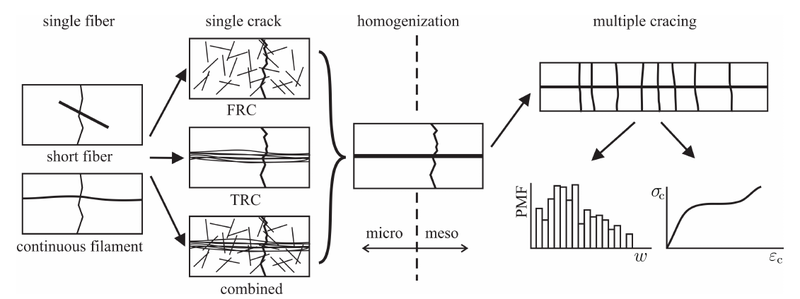
\includegraphics[width=0.9\textwidth]{fig/Lecture01/composite_types.png}
	\caption{Examples of considered brittle-matrix composites}
	\label{fig:composite_types}
\end{figure}


\mnote{Considered types of composites}
The explained concepts are applicable to the following types of composites exemplified in Fig.~\ref{fig:composite_types}
\begin{description}
\itemsep=-1mm
\item[A: Continuous, discrete reinforcement elements] which are explicitly placed by design at a given location. 
This represents the bar reinforcement in steel-reinforced concrete or reinforcement using CFRP or GFRP bars. 
The cross-sectional area of individual bars is of the order of centimeters.
\item[B: Dispersed continuous reinforcement] denoting fine meshes and grids of reinforcement, for example textile fabrics or mats. 
This reinforcement represents a layer acting in two dimensions. Profiled textiles and prefabricated three-dimensional structures 
are also included in this category. 
\item[C: Discontinuous, dispersed short fiber reinforcement] with randomly distributed and oriented fibers. This type of reinforcement is a part of the concrete mixture.
\end{description}

The behavior of the three types of composites is certainly different and should be 
considered complementary. Each of them is associated with different type of behavior 
and different manufacturing methods so that they are suitable for different 
types of applications in architecture and structural engineering.
The description of their behavior, even though quantitatively different, 
can be boiled down to the same key mechanism, the interacting matrix cracking 
and debonding of matrix and reinforcement.

\mnote{Material design}
The detailed knowledge provides possibility to design a material structure combining all the mentioned types of composite. By combining different types of concrete mixtures, fiber cocktails, textile reinforcement and discrete bar reinforcement the design space becomes huge. The level of initial stiffness, the ductility, the ultimate tensile strength can be modified as desired.

\mnote{Research method}
Finally, the course will present the concepts following the scientific practice of material research clarifying the notions of experimental design, model calibration, model validation, parametric study, sensitivity analysis.  

\section{Scope and structure of the course}

\mnote{Three structural levels}
This course aims to present this knowledge by three 
cases of macroscopic, structural behavior.
In the first part of the course, we look into the debonding process 
between two material components on an example of a pullout test. 
In the second part,
we will describe the crack propagation in concrete by considering
a bending test and its modifications. In the third part,
we describe the interaction of cracking and debonding using 
tensile, and bending test of a composite specimen.

\mnote{Three perspectives}
In each of these three parts we will use 
these perspectives of observation. 
The subjective perspective will be used
to evaluate the experimental observation
of the structural response, i.e. the test results.
In the second perspective, a model of the observed
structural behavior will be presented and will be used to "play around" with the experiment asking the question:
\begin{quote}
\textit{What happens when something gets changed?}
\end{quote}
The third, most objective perspective will then 
regard the process from the perspective of a material point or zone.

\mnote{Putting it together}
By following this scheme, we will develop a general and in-depth understanding 
of material and structural behavior applicable to wide range of
materials. Except of traditional, steel-reinforced concrete
we will apply it to innovative composite materials using 
nonmetallic reinforcement materials, like carbon bars.
In the last part of the course, we will sketch a design of a structure 
that exploits the material quasi-ductile behavior of cementitious composite 
in a safe and economic way. We will discuss the aspects of the structural behavior, 
in view of stress-redistribution and ductility both at the level of a cross 
section and at the level of the whole structure. Then, we will compare 
this view with the linear-elastic analysis and prediction of ultimate failure. 
This discussion will provide the basis for understanding of 
structural redundancy and safety assessment.



\section{Example applications of cementitious composites}

\mnote{Application domain}

The application domain of brittle-matrix composites
is still rapidly growing. Except of the traditional domain of steel-reinforced concrete (reinforcement of type A), innovative composites applying non-metallic reinforcement are included. Lightweight structural elements, like thin-shells provide appealing features, like low material consumption and high durability. 

Many examples of structures applying also non-metallic reinforcement already exist and a number of them has been realized in the framework
of research projects at the Institute of Structural Concrete of the RWTH Aachen University. On the one hand, thin walled 
shells made of textile-reinforced concrete \ref{fig:shells} applying the reinforcement layout of type B 
demonstrate the feasibility and the specific features of the new composite materials. On the other hand 
an application of CFRP as bar reinforcement (type A) has realized in collaboration is shown in Fig.~\ref{fig:albstadt}.

\mnote{Design rules for new composites}
However, their broader applicability is hindered by a missing support for engineering design rules. 
The traditional design codes cannot be simply adopted, because of qualitative differences in their material behavior. Application of these new types of composites requires the development of new codes and assessment methods from scratch. Standardization of testing methods is also an important issue.


\begin{figure}[tb]
\centering
\begin{subfigure}{0.45\linewidth}
	\centering
  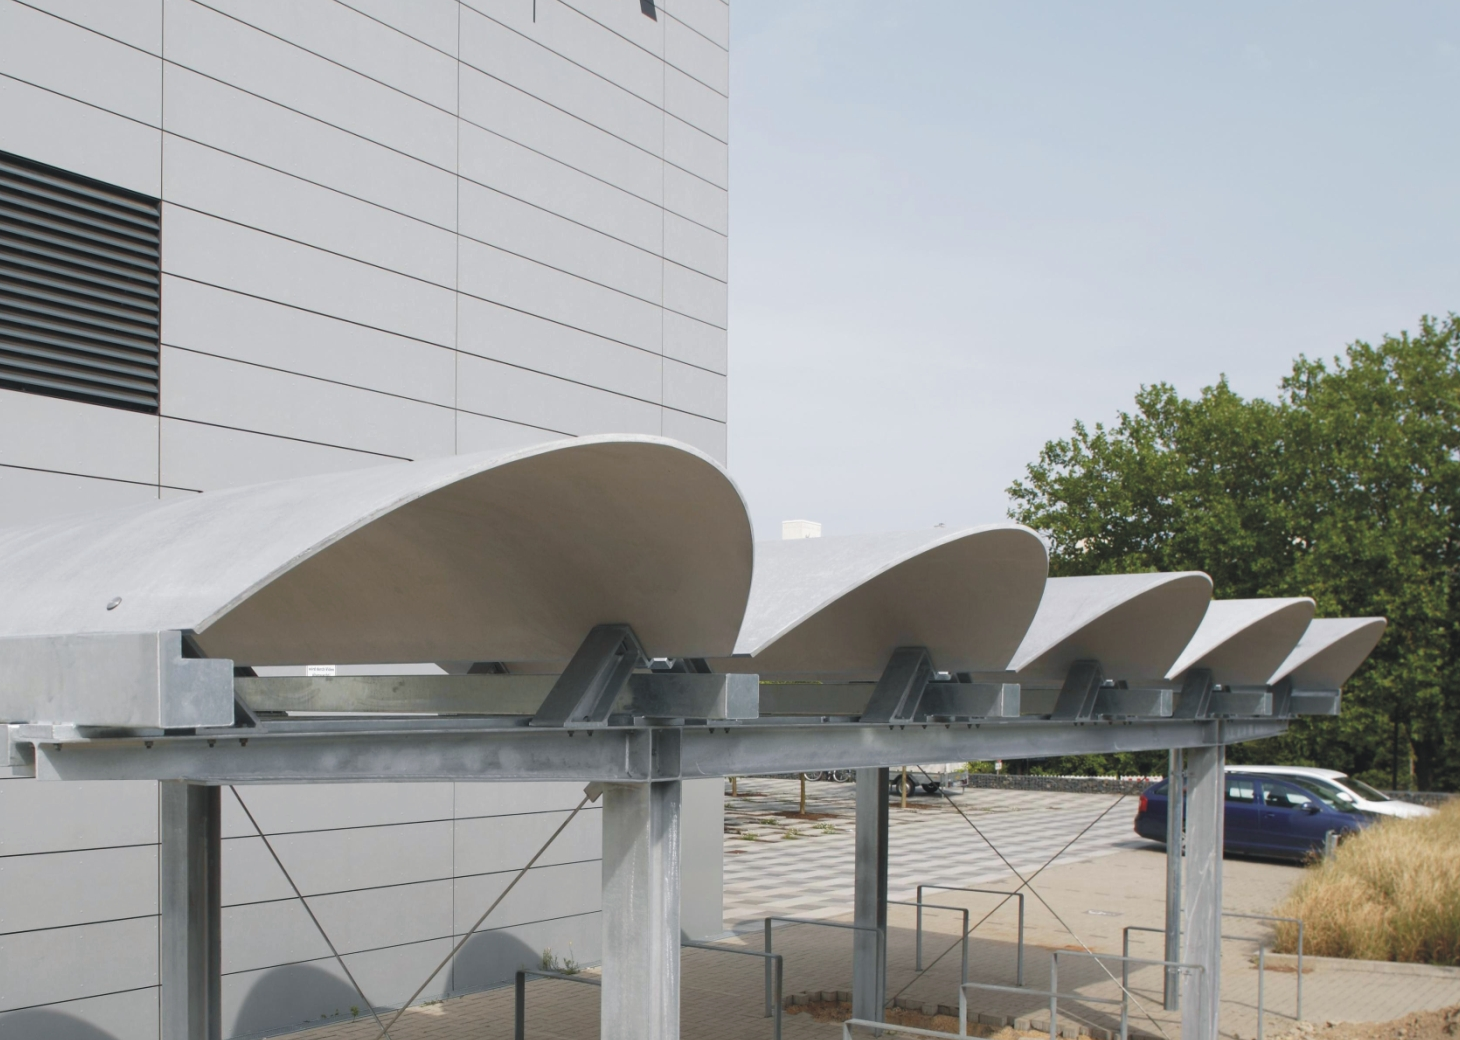
\includegraphics[height=5cm]{fig/Lecture01/vault_shell.png}
	\caption{Campus Melaten, Aachen}
	\label{fig:vault_shell}
\end{subfigure}
\hspace{0.5cm}%
\begin{subfigure}{0.45\linewidth}
	\centering
  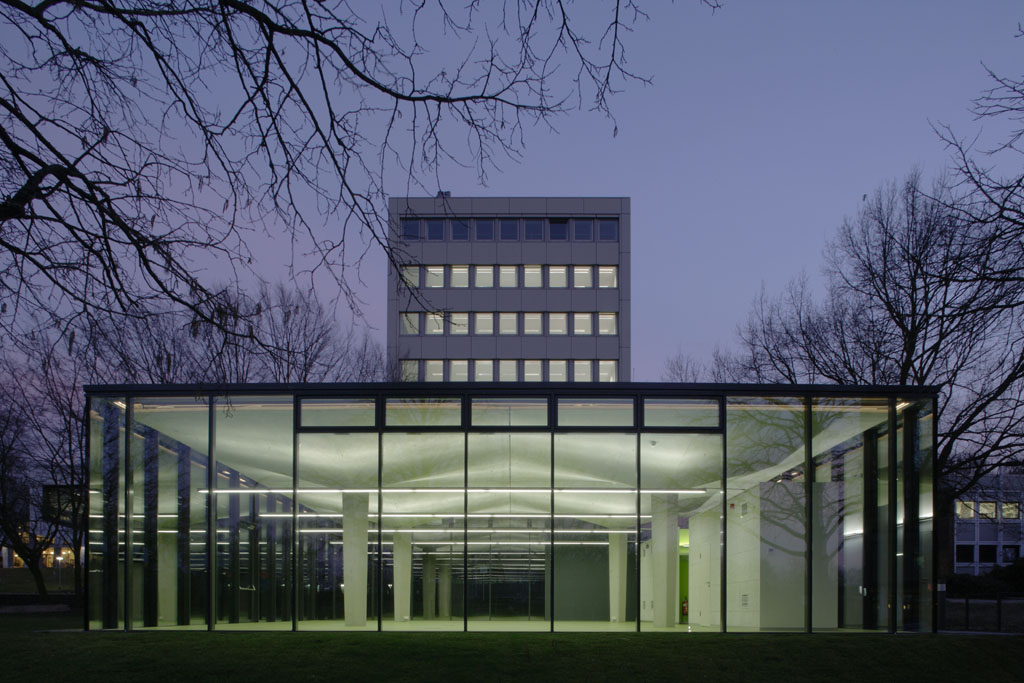
\includegraphics[height=5cm]{fig/Lecture01/t3.png}
	\caption{T3 Pavillon, RWTH Aachen}
	\label{fig:t3_pavillon}
\end{subfigure}
\caption{Examples of textile-reinforced concrete shells}
\label{fig:shells}
\end{figure}
\begin{figure}
\centering
  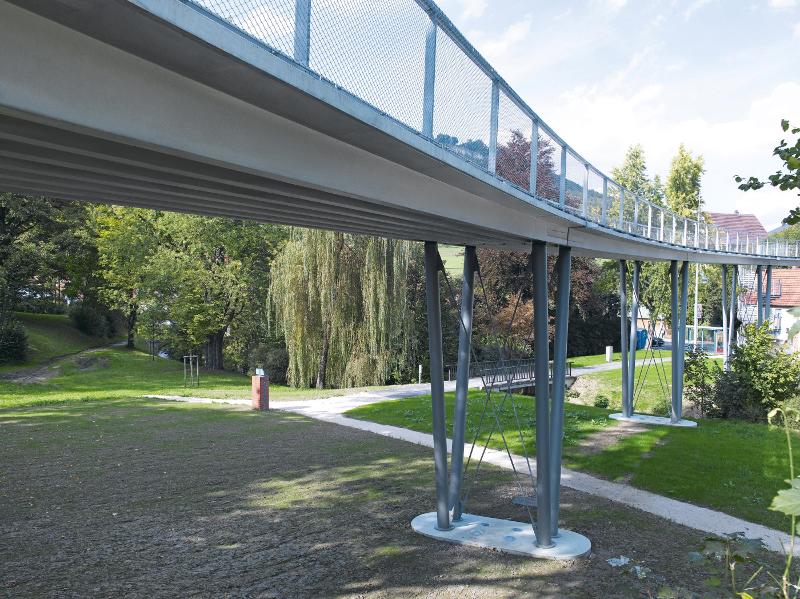
\includegraphics[height=5cm]{fig/Lecture01/trc_alpstadt.png}
	\caption{TRC bridge, Albstadt}
	\label{fig:albstadt}
\end{figure}

Except of the mentioned cases, the methods described in this course are also relevant for the analysis of FRP sheet lap joints applied for retrofitting of aging structures. At the same time, they are relevant also for application of TRC as a  strengthening layer of existing structures, such as bridges.

\section{BMCS Tool Suite}

\mnote{Interactive demonstration of the taught concepts}
The BMCS Tool Suite is a package of specialized programs that can be used by the course participants to study particular effects of the material- and structural behavior. The idea is to show the students an implemented model of a particular test setup in an interactive form first so that they can perform some virtual experiments. After showing a few examples of what kind of behavior the model can describe, the theory behind the model can be explained with a clear specification about the purpose and assumptions related to the model. 

\mnote{Open-source bundle for scientific computing}
The BMCS Tool Suite has evolved from several years of research in the field of material modeling of brittle-matrix composites. This development has been carried out using open-source scientific computing libraries developed in Python language. The computing environment consists of several hundreds of open-source, free libraries. For convenience, they are packaged within the Canopy software bundle, which is free for academic purposes. The Installation of Canopy can easily be performed on all existing platforms including, Windows, Mac and Linux operating systems. 

\mnote{Role of the BMCS models in the course}
The models implemented in BMCS-Tool can be installed on any computer platform. The implementations are computationally efficient, they are equipped with a simple interactive user interfaces that allows the students to start with a study of a problem at hand from scratch without any prerequisite knowledge. At the same time, students have a chance to learn modern implementation concepts of models during the course using a high-level programming language with a large expressive power. Just to mention an example, this environment enables us to implement a finite-element solver of a pull-out problem on some 15 lines of code, which is very closely related to the mathematical description of the model. These features make this environment ideally suited for the teaching concept followed within the BMCS course. 

The installation guide to the \lstin{Canopy} and \lstin{BMCS} is provided at the moodle page of the course 
and can be directly accessed
\href{https://store.enthought.com/downloads}
{here} 

\section{Warm-up exercises}

\begin{bmcsex}{Material stiffness of a composite  cross section}{e11_rule_of_mixture}

What is the initial stiffness of a reinforced concrete cross section shown in Fig~\ref{FIGCrossSection} with the thickness of 10~mm and width of 100~mm.
The cross-section is reinforced with 6 layers of textile fabrics made of CAREP3300 specified in Table~\ref{t:cross_sections}.

Evaluation script is available \href{https://moodle.rwth-aachen.de/pluginfile.php/263167/mod_folder/content/0/Example%201.1%20-%20Calculate%20the%20elastic%20stiffness%20of%20the%20composite.ipynb?forcedownload=1}{here}

\begin{lstlisting}
A_roving = 1.84 # [mm**2] 
n_layers = 6 # - 
spacing = 25.77 # [mm] 
thickness = 10 # [mm] 
width = 100 # [mm] 
E_carbon = 240000 # [MPa] 
E_concrete = 28000 # [MPa]

A_composite = width * thickness 
n_rovings = width / spacing 
A_layer = n_rovings * A_roving 
A_carbon = n_layers * A_layer 
A_concrete = A_composite - A_carbon 
E_composite = (E_carbon * A_carbon + E_concrete * A_concrete) / (A_composite)

print ('E_composite', E_composite , 'MPa') 
\end{lstlisting}


\end{bmcsex}

\begin{figure}[tb]
	\centering
  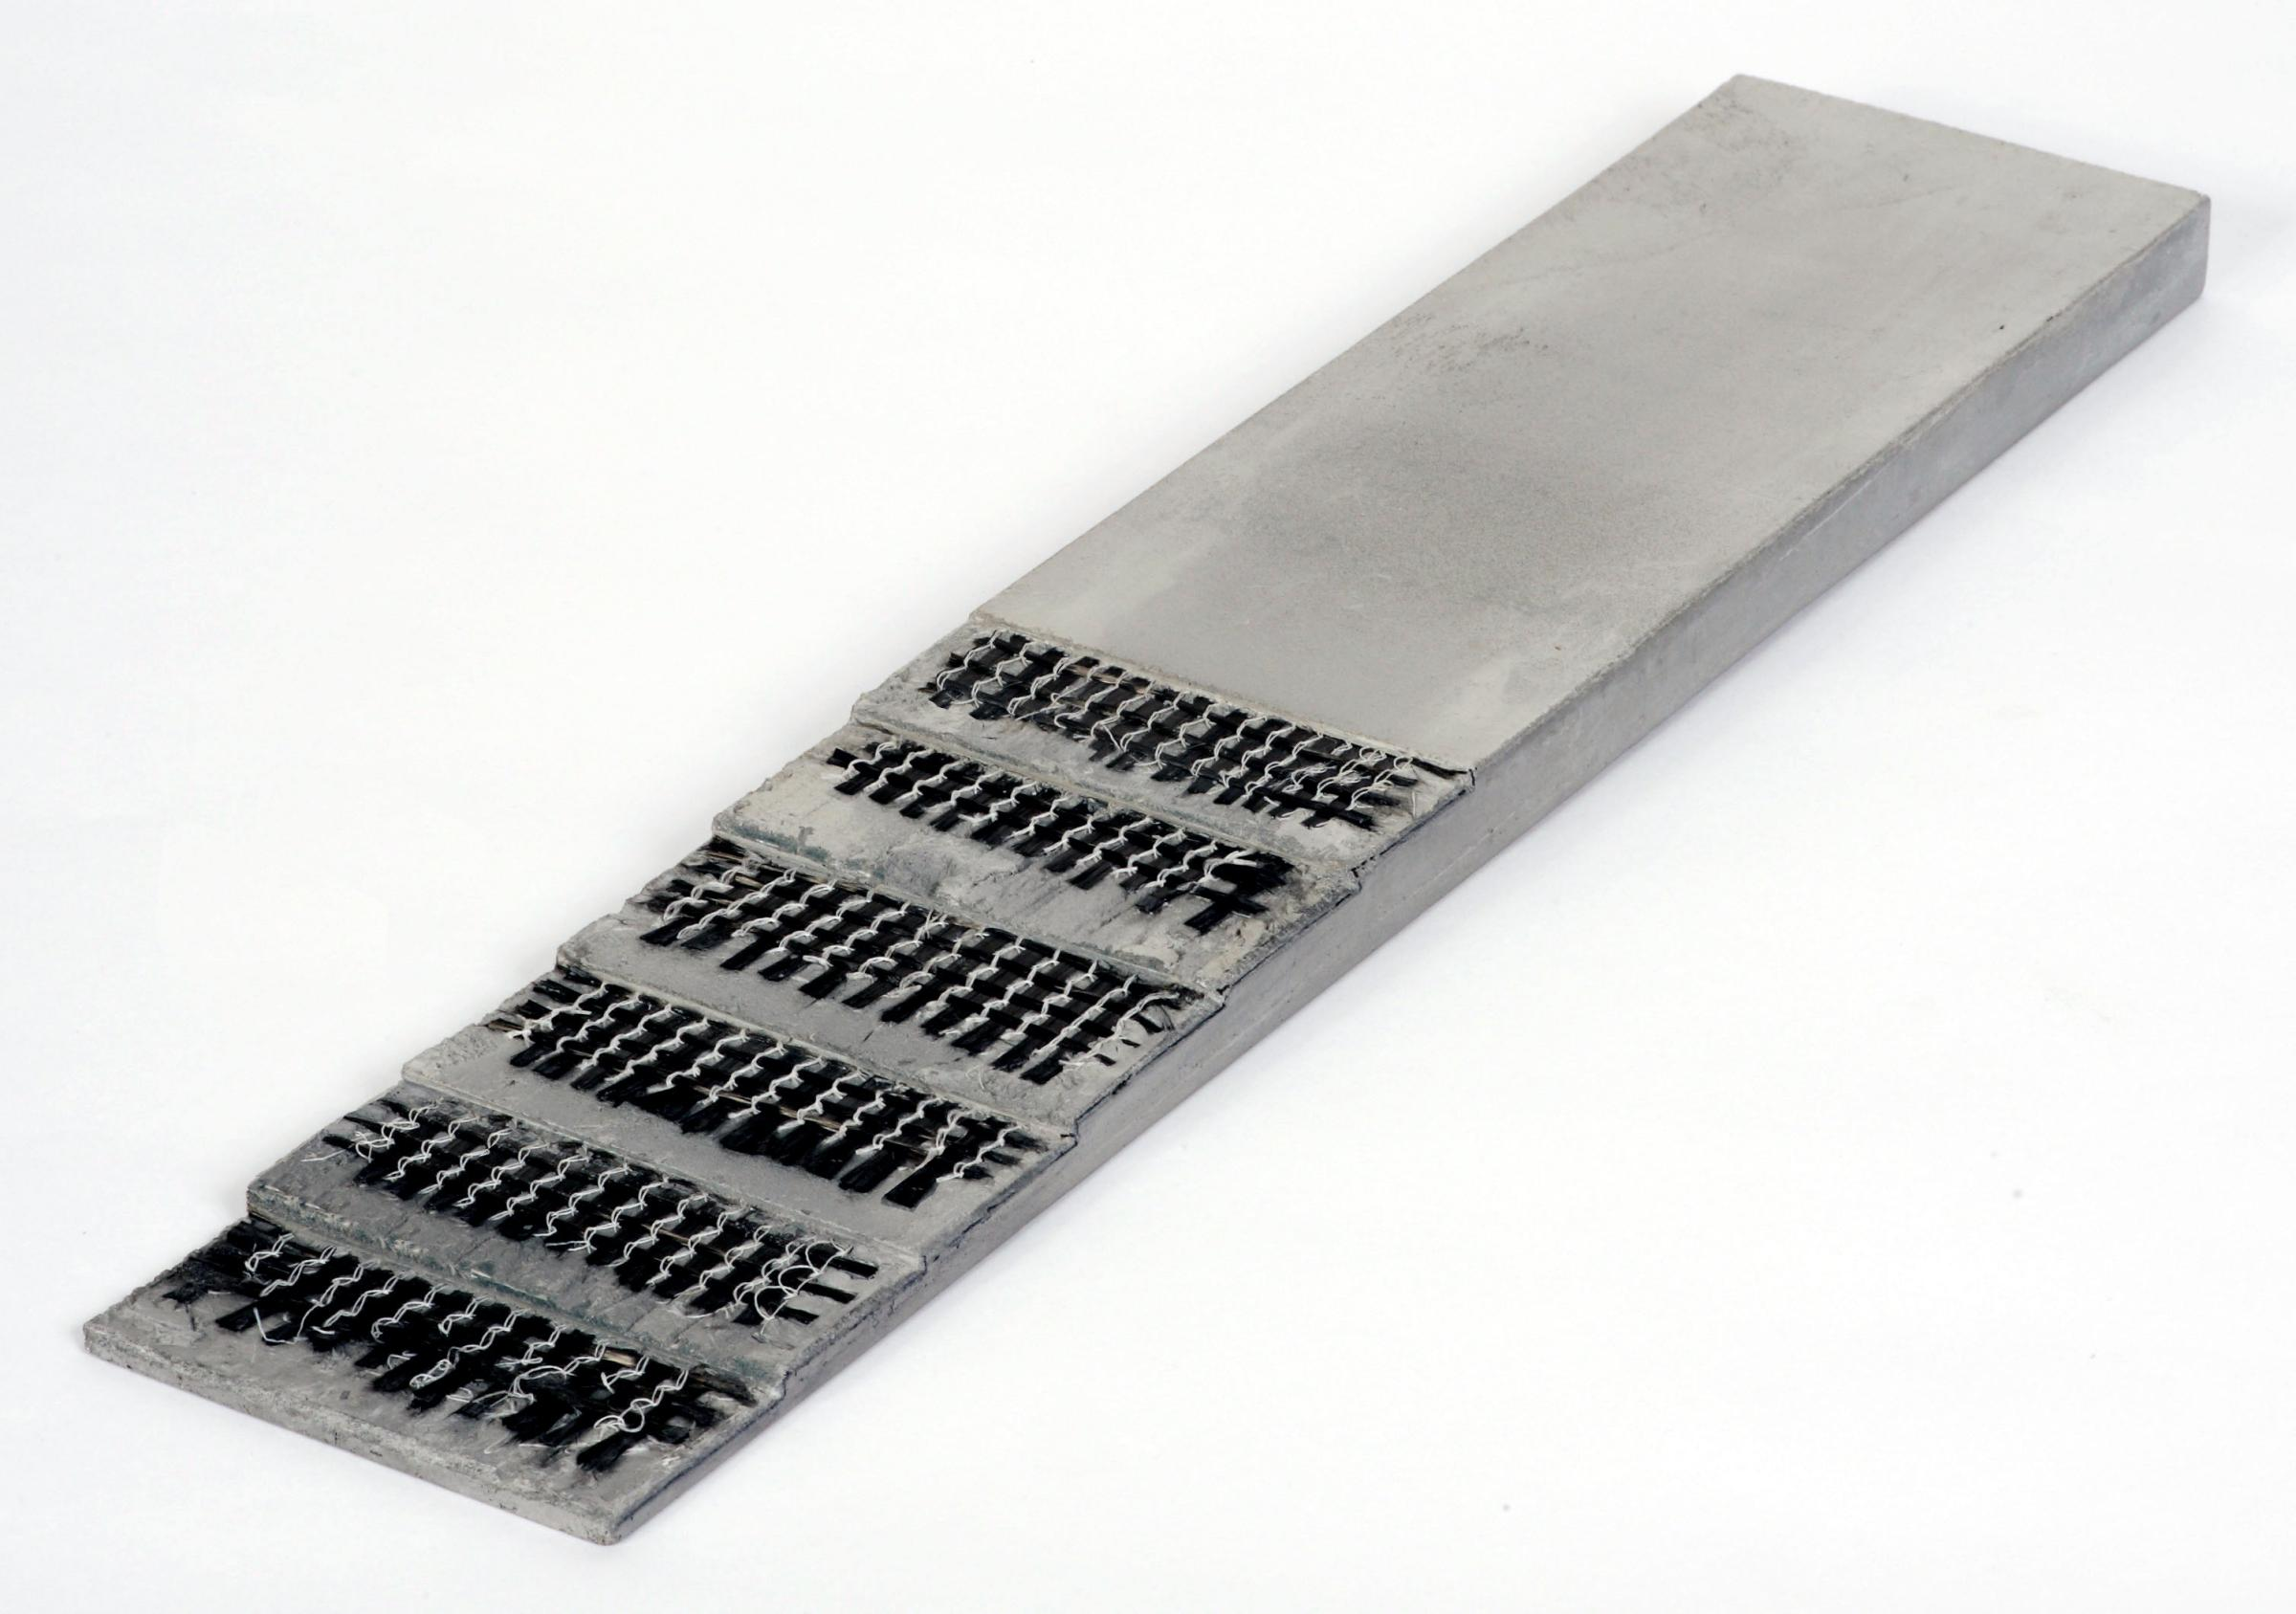
\includegraphics[width=0.4\textwidth]{fig/Lecture01/TRC-example.png}
	\caption{Examples of material parameters of textile-fabrics reinforcement}
	\label{FIGCrossSection}
\end{figure}

\begin{bmcsex}{Volume fractions and reinforcement ratio}{e12_volume_fraction}
Given a concrete matrix with $E$ modulus of 28~GPa, carbon reinforcement of 
200~GPa, and glass textile fabrics with of 70~GPa  ... design a material cross section  
with the overall stiffness of 45~GPa.

Evaluation script is available \href{https://moodle.rwth-aachen.de/pluginfile.php/263167/mod_folder/content/0/Example%201.2%20-%20Calculate%20the%20cross%20sectional%20area%20of%20a%20component%20to%20achieve%20a%20desired%20stiffness.ipynb?forcedownload=1}{here}

\begin{lstlisting}
A_concrete = 50 * 50 # [cm**2]
E_concrete = 28 # [GPa]
A_carbon = 0.08 * A_concrete # [cm**2]
E_carbon = 200 # [GPa]
A_glass = 0.184 * A_concrete # [cm**2]
E_glass = 70 # [GPa]
A_composite = A_concrete + A_carbon + A_glass
E_composite = (
  (E_concrete * A_concrete + E_carbon * A_carbon + E_glass * A_glass) / A_composite
)
print('E_composite', E_composite)
\end{lstlisting}

\end{bmcsex}

\begin{table*}[tb]
 \centering
 \caption{Cross sections characteristics; parameters of performed tests in boldface font, derived values in normal font}\label{t:cross_sections}
 \begingroup\setlength{\fboxsep}{0pt}
%\colorbox{lightgray}
{\footnotesize
 \begin{tabular}{ m{3.2cm} m{2cm} m{2.1cm} m{2.0cm}  m{2.0cm} m{2.0cm}  }
    \toprule
    Label
    & Material
    & Area 
    & Grid spacing
    & Stiffness
    & Strength (characteristic)
    \\ 
  \hline 
    &     
    & [mm$^2$]
    & [mm]
    & [MPa]
    & [Mpa]
    \\ 
%     \hline
%     S-Q150
%     & steel
%     & 7e-5
%     & 150
%     & 210000
%     & 350
%     \\ 
%   \hline
%     CAR-2400
%     & carbon
%     & 5e-7
%     & 8.3
%     & 240000
%     & 2400 
%     \\
   \hline
    CAR-EP3300
    & carbon/proxy
    & 1.84
    & 25.77
    & 240000
    & 3500
    \\
   \hline
    solidian GRID Q95
    & carbon/proxy
    & 3.62
    & 36.0
    & 240000
    & 3200
    \\ \bottomrule
 \end{tabular}%
}\endgroup
\end{table*}

\end{document}


